\chapter{Common Scrambling Algorithm} \label{ch:CSA}
The Common Scrambling Algorithm (CSA) is currently the most commonly 
used encryption algorithm for encryption of video-streams, in the DVB 
context. The CSA uses a combination of a block cipher, taking an input 
of a 64-bit block, and a stream cipher. Both of the ciphers use the 
same key, which means that the entire system uses the same key. This 
means that the complete algorithm would break if the key would be 
recovered, as long as the person recovering the key knows what the 
decryption algorithm looks like. Using the same key does on the other 
hand allow us to easily change the key at regular intervals. 
\citep[pp. 271--272]{WeiLi:2007}

CSA has been the official scrambling method for protecting DVB content 
 since may 1994. CSA was to be easily implemented in hardware and hard 
to implement in software to, among other reasons, make 
reverse-engineering of the algorithm difficult \citep{DVBScene:2013}.

There are two versions of the DVB-CSA, CSA1 and CSA2, where the 
key-length is the only difference.
\citep[p. 23]{DVBScene:2013}

\section{The need for a new standard}
The DVB-CSA standard offers short-term protection, while it assumes 
content is viewed in real time and not stored. Due to the development 
of how content has come to be consumed during recent years, the focus 
has shifted to primarily being able to distribute content across homes. 
As a result of this, functionality needs to be changed from securing 
the delivery of content, to securing the content. \citep{Farncombe}

Another thing to bear in mind is the fact that more CPU-based units, 
such as smart-phones, tablets and computers are used to access contents 
now more than ever. In order to allow for descrambling on CPU-based 
units, a software-friendly scrambling algorithm might be needed.

\section{Layout of the CSA}
The CSA consists of a block cipher and a stream cipher which are 
connected in sequence \citep[p. 271]{WeiLi:2007}. The block cipher 
reads blocks of data, each consisting of 64-bits, which are run in 
CBC-mode (see section \ref{sec:BlockCipher}). The block cipher 
processes these blocks of data in 56 rounds. The output of the block 
cipher is sent to the stream cipher, where additional encoding is 
performed. The first block of data sent from the block cipher to the 
stream cipher is used as an IV for the stream cipher. Therefore it is 
not encoded at this point, in the stream cipher. 
\citep{DVBAnalysis:2006}

\section{Security}
One of the problems associated with control word distribution is that 
control word sharing has become rather common \citep{Farncombe}. This 
is possibly since the control words are sent in the clear between the 
smart card and the STB, meaning that a user might grab the clear 
control word during transmission and redistribute it over the internet. 
This has become a financial problem for content distributors, since 
people have stopped paying for the content that they are watching.

One way of dealing with control word sharing is to decode the encrypted 
control word on the CI system, and then encrypt it once again on the CI,
before sending it to the STB. The latter key is setup between the CI 
system and the STB through a one time sychronization. This means that 
users are not able to grab the clear control word and redistribute it. 
\citep[pp. 12--13]{HIS:2011}

Another security issue that you need to think of when designing the 
hardware, to prevent content theft, is to make sure that no contacts 
are ever accessible from the top layer of the circuit board. This is 
due to the fact that people would be able to connect hardware to the 
board and download the material that way, if they were. 
%%%%%%%%%%%%%%%%%%%%
%\Warning[Source]{Except from Patrik Lantto}
%%%%%%%%%%%%%%%%%%%%
There also exists a need to be aware of people trying to break the 
algorithm through forced ways, as well as CW sharing and hardware 
methods of stealing content.

\subsection{Breaking the CSA}
There are a few standard ways to try to break ciphers. The most common 
ones are the brute force-, known plaintext-, chosen plaintext- and 
birthday attacks. You choose what method to use depending on what design
of the cipher is. The most relevant ones, in the context of the CSA, 
will be explained in the following subsections. 
\citep[pp. 31-34]{Schneier:2003}

\subsubsection{Brute force}
The number of unique keys that can be extracted depends solely on the 
length of the key. The number of combinations corresponds to the 
largest number, plus one. The formula for the largest possible number 
obtainable, when working on keys represented as binary numbers, where 
the key-length is represented by the letter n, can be viewed in equation
\ref{eq:num}. Note that the key-length is in bit size.

\begin{equation} 
  \text{Largest possible number} = 2^{n} - 1
  \label{eq:num}
\end{equation}

Since the CSA uses keys consisting of 64-bits (8 bytes), this gives us 
18.5 Quintillion ($10^{18}$) possible keys. However, \emph{byte} 3 and 
7 are often used as parity bytes in CA systems, which leads to only 48 
bits being used in the key.  This can be seen in figure 
\ref{fig:blockcipher}. 48 bits on other hand would lead to $2^{48}$ 
combinations, which corresponds to 281 Trillion ($10^{12}$) possible 
unique keys. 

Testing a million keys per second is about what is possible through a 
modern x86 processor using software methods 
%%%%%%%%%%%%%%
%\Warning[Todo]{How did I get this number?}, which means it would take 
%%%%%%%%%%%%%%
roughly 3258 days to force brake the keys, which translates into 
roughly 8.8 years. The calculations are done in equation \ref{eq:keys} 
through \ref{eq:days}. \citep{Breaking:2012}

Number of unique keys, for a 48-bit key:
\begin{equation}
  2^{48} = 2,814749767*10^{14} \text{ keys}
  \label{eq:keys}
\end{equation}

By dividing by the number of tested keys per second, the number of 
seconds to test all the keys will be found:
\begin{equation}
  281*10^{12} / 10^{6} = 281,4749767*10^{6} \text{ seconds}
  \label{eq:seconds}
\end{equation}

By substituting seconds, with day * (seconds/day), the number of keys 
per days is found insteal:
\begin{equation}
  281,4749767*10^{6} / 86400 = 3257,8 \text{ days}
  \label{eq:days}
\end{equation}

\begin{figure}[h!]
  \begin{center}
    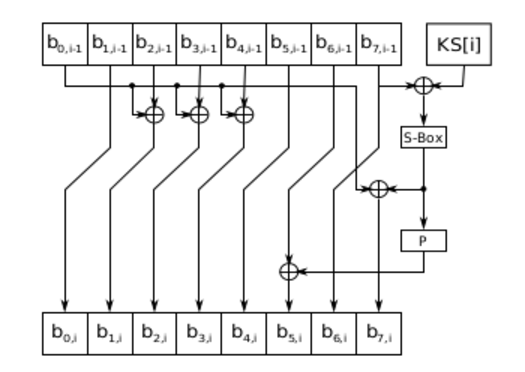
\includegraphics{blockcipher}
  \end{center}
  \caption{Number of bits in key used}
  \label{fig:blockcipher}
\end{figure}

Moreover, systems need to change the key at least every 120 seconds 
\citep{Simpson:2009}. Changing the key every second minute would mean 
that 140 trillion keys would need to be scanned per minute, to cover 
the most of the keys in the two minutes available before the key is 
changed. However, most systems issues new keys between every 10th - 
120th second, which means that for some systems 28.1 trillion keys need 
to be scanned per second \citep{Wirt:2004}.

It is possible to use dedicated hardware and FPGA implementations to 
speed this up, through hardware accelerations and other methods. This 
could make it possible to scan through 2.8 trillion keys per second, 
just barely allowing us to be certain to find the key in two minutes. 
Even so, the key could just be changed more frequenctly than every 
second minute. As such, the brute force method of is not a reasonable 
method to obtain the key.

\subsubsection{Known plaintext attack}\label{sec:kpa}
The known plaintext attacks are performed to figure out the key. What 
is interresting is that this kind of attack only is applicable for 
symmetric ciphers. That means that the known plaintext attack can not 
be used to retrieve the secret key during public-key encryption 
(section \ref{ch:public}). The key can then be used to decrypt 
following ciphertexts. To perform this kind of attack, a known 
plaintext-ciphertext pair is needed. You can try to find the key if 
you have the both of them. This is done by identifying ciphertexts 
known to correspond to zero-filled plaintexts, when trying to break the 
CSA \citep{Breaking:2012}. Memories are then filled with precalculated 
keys, which are used to find which key the current plaintext-ciphertext 
pair corresponds to. This method is supposed to recover a key in 
roughly 7 seconds with a 97\% certainty according to 
\citet{Breaking:2012}.
